\section{Proofs}\label{app:proofs}
Throughout, $\Delta_j=x_j-s_j\ge0$, $h_j=u_j-s_j\ge0$.

\paragraph{Proof of \cref{p:mean}.}
$t$ is first iff $\sum_jx_j>\max_{i\ne t}\sum_jS_{ij}$, i.e.\ $\sum_j\Delta_j>G$. Since $\sum_j\Delta_j\le\sum_jh_j$, the plan exists iff $\sum_jh_j>G$. Every plan with total gain $>G$ is feasible, so $\inf\sum_j\Delta_j=G$ (not attained). Touching $k$ tasks yields at most the sum of the $k$ largest headrooms, which must exceed $G$; filling the largest headrooms first attains it, giving $\Bst$ and $\Bst\ge G/\max_jh_j$. For $D$ the problem is $\min\sum_jN_j\Delta_j$ s.t.\ $\sum_j\Delta_j>G$, $0\le\Delta_j\le h_j$, a fractional knapsack whose optimum fills tasks in increasing $N_j$. \qed

\paragraph{Proof of \cref{p:quantile}.}
$f_r(x)>\theta$ iff at least $r$ coordinates of $x$ exceed $\theta$. Initially $a$ do. Raising a coordinate that already exceeds $\theta$ does not change the count and raising one that does not can increase it by one only if it is pushed above $\theta$, which needs $u_j>\theta$. So at least $r-a$ coordinates with $s_j\le\theta$ must be touched (fewer touches leave the count $\le r-1$, hence $f_r\le\theta$), and $r-a$ suffice when enough eligible tasks exist; each is raised to $\theta+\epsilon$ at cost $w_j(\theta-s_j+\epsilon)$ and the cheapest $r-a$ are chosen. Beating $\theta=\max_i f_r(S_i)$ is equivalent to beating every rival. \qed

\paragraph{Proof of \cref{p:margin}.}
For rival $i$ let $M_i(x)=M_i(s)+\sum_j\phi_{ij}(x_j)$ with $\phi_{ij}$ non-decreasing, $\phi_{ij}(s_j)=0$ (the margin is a sum over tasks of terms in which only $x_j$ varies, and raising $x_j$ can only turn a loss into a tie/win or a tie into a win). Let $\gamma_{ij}=\phi_{ij}(u_j)$ be the maximal gain. Any plan that beats rival $i$ must satisfy $\sum_j\phi_{ij}(x_j)>-M_i(s)$ hence touch at least as many tasks as the shortest prefix of the $\gamma_{i\cdot}$ sorted decreasingly that exceeds $-M_i(s)$; this is $\Bst_i$ (attained for the single rival by lifting to the ceiling). A plan for the full problem beats all rivals, so $\Bst\ge\max_i\Bst_i$. The per-task bounds: for Condorcet $\phi_{ij}\le\mathrm{sign}(1)-\mathrm{sign}(-1)=2$; for plurality $t$ gains at most one win and $i$ loses at most one, so the margin changes by $\le2$; for Borda $t$ gains at most $m-1$ points on a task and $i$ loses at most one. \qed

\paragraph{Proof of \cref{p:sep}.}
(a) One rival with scores $0.5$ everywhere; target $0.5-\delta$ everywhere, $\delta=\frac{1}{4(n-1)}$. Mean: $G=n\delta<0.5+\delta=h_j$ for all $j$ (equivalent to $(n-1)\delta<0.5$), so one task suffices. Median: $\theta=0.5$, $a=0$, $r=\frac{n+1}2$, hence $\Bst=\frac{n+1}{2}$ by \cref{p:quantile}.
(b) Rival $0.5$ everywhere; target: $k=\frac{n-1}2$ tasks at $0.51$, one task at $0.49$, the other $k$ tasks at $0$. Then $a=k$ and $\Bst_{\text{median}}=r-a=1$ (lift the $0.49$ task). The mean gap is $G=\frac n2-0.51k-0.49=0.245n-0.235$, the $k$ zero tasks have headroom 1 (the largest), so $\Bst_{\text{mean}}=\lfloor G\rfloor+1=\lfloor 0.245n-0.235\rfloor+1$ whenever $G<k$. Both instances are verified numerically for $n\in\{5,9,21,57\}$ in \texttt{src/analysis\_theory.py} (output in \texttt{out/theory\_summary.txt}). \qed

\paragraph{Proof of \cref{p:convex}.}
The mean problem is $\min\sum_jc(\Delta_j)$ s.t.\ $\sum_j\Delta_j\ge G$, $0\le\Delta_j\le h_j$. It is strictly convex with a unique solution; KKT gives a multiplier $\lambda>0$ ($G>0$) with $c'(\Delta_j)=\lambda$ whenever $0<\Delta_j<h_j$, $c'(\Delta_j)\le\lambda$ if $\Delta_j=0$. Since $c'(0)=0<\lambda$, $\Delta_j=0$ with $h_j>0$ would contradict stationarity (raising $\Delta_j$ lowers the Lagrangian). Hence $\Delta_j>0$ for every $j$ with $h_j>0$; for $c(\Delta)=\Delta^2$ the solution is $\Delta_j=\min(h_j,\lambda/2)$. For order statistics, each pushed task must reach $\theta$ whatever the convexity, and an increasing $c$ makes the $r-a$ smallest gaps optimal. \qed

\section{Solvers and validation}\label{app:val}
\textbf{0--1 program.} For Borda, plurality and Condorcet and a target $t$, a rival is \emph{binding} if its margin over $t$ is $\le0$ (margins never decrease, so non-binding rivals stay beaten). Variables $y_{jl}\in\{0,1\}$ select for task $j$ a \emph{level} $v_{jl}$: the distinct rival scores in $[s_j,u_j)$ (placing $t$ at $v+\epsilon$ beats exactly the rivals with score $\le v$); for plurality the only level is just above the column maximum. Constraints: $\sum_ly_{jl}\le1$; for each binding rival $i$, $\sum_{jl}\mathrm{inc}_{i,jl}y_{jl}\ge\mathrm{need}_i$, where $\mathrm{inc}$ is the exact change in margin (for Borda the change in $t$'s points plus the loss of $i$'s points on that task; doubled so that half-points are integral). Objectives: $\sum y$ (breadth), $\sum(v-s_j)y$ (points) and $\sum N_j(v-s_j)y$ (data). HiGHS (via SciPy) is run with relative gap $10^{-9}$ and a 120\,s limit; the status of every solve is stored in the output CSVs (all runs terminated with status 0 = optimal; check with \texttt{grep} on the \texttt{status} column). Plurality shares are fractions, so rows are scaled by $10^4$ and require margin $\ge10^{-4}$ (conservative for margins below $10^{-4}$, which do not occur).
\textbf{Verification.} After solving, each of the three plans is applied to the leaderboard and the rule is recomputed from scratch; the code asserts that the target is strictly first (tolerance $10^{-11}$), $x\ge s$ and $x\le\max(u,s)$.
\textbf{Brute-force test} (\texttt{tests/test\_core.py}; output \texttt{out/test\_log.txt}): 300 random instances ($m{=}6$, $n{=}5$, scores on a 0.1 grid so ties are frequent, random continuous ceilings, random weights) for mean, median, $f_1,f_2,f_5$, Borda, plurality, Condorcet: $\Bst$ equals exhaustive search over subsets lifted to ceilings in every feasible case (feasibility also agrees), and $\Pst$, $\Dst$ equal exhaustive search over candidate levels (for the mean, $\Pst=G$). 100 instances for the even-$n$ median.
\textbf{Ties at ceilings.} A plan may place $t$ exactly at a rival's score (a tie) only at a ceiling; the solvers ignore such ties (conservative). No cell of either board equals 1, and caps $s_j+g$ are continuous.
\textbf{Even-$n$ median.} For $n=2k$ the median is the average of the $k$-th and $(k{+}1)$-th largest; $t$ wins iff $d_k+d_{k+1}>2M$. We enumerate the $k$-subset lifted to level $\alpha$ and one further task lifted to $2M-\alpha$ over all breakpoints $\alpha$ (exact for small $n$); breadth by subset enumeration.

\section{Additional results}\label{app:extra}
\begin{table}[h]
\caption{Open LLM Leaderboard (all 4{,}576 models), top-21 targets by the official mean: feasibility (fraction reaching first) and median breadth among all targets (infeasible ones counted as missing) at three per-task gain caps $g$ in normalised points.}
\centering\small\begin{tabular}{@{}lrrrrrr@{}}\toprule
 & \multicolumn{2}{c}{$g=5$} & \multicolumn{2}{c}{$g=20$} & \multicolumn{2}{c}{$g=100$ (ceiling)}\\
 Rule & feas. & $B$ & feas. & $B$ & feas. & $B$\\\midrule
mean & 0.65 & 6 & 1.00 & 2 & 1.00 & 1\\
median & 0.75 & 1 & 1.00 & 1 & 1.00 & 1\\
borda & 0.75 & 2 & 1.00 & 1 & 1.00 & 1\\
plurality & 0.15 & 2 & 1.00 & 2 & 1.00 & 2\\
condorcet & 0.30 & 3 & 1.00 & 3 & 1.00 & 3\\
\bottomrule\end{tabular}

\end{table}
\begin{table}[h]
\caption{Stability of rank-group medians under evaluation noise (200 binomial replicates, seed 4; ranks recomputed in each replicate).}\label{tab:noisebins}
\centering\small\begin{tabular}{@{}llrr@{}}\toprule
Rule & ranks & $B^\ast$ median [95\% interval] & $D^\ast$ median [95\% interval]\\\midrule
mean & 4-10 & 5.0 [4.0, 6.0] & 178 [142, 220]\\
mean & 11-30 & 10.0 [9.0, 11.0] & 455 [420, 506]\\
mean & 31-79 & 21.0 [20.0, 22.0] & 1276 [1208, 1342]\\
median & 4-10 & 6.5 [3.5, 10.0] & 15 [5, 35]\\
median & 11-30 & 14.0 [12.0, 17.0] & 89 [65, 119]\\
median & 31-79 & 26.0 [25.0, 27.0] & 392 [348, 450]\\
\bottomrule\end{tabular}

\end{table}
\begin{figure}[h]
\centering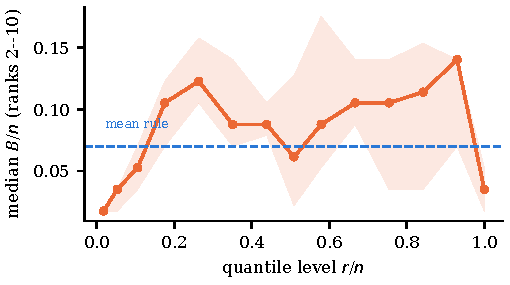
\includegraphics[width=.5\textwidth]{figs/fig_quantile.pdf}
\caption{Order-statistic family on HELM (ceiling): median $B/n$ over targets with initial rank 2--10 versus quantile level $r/n$ ($r$-th largest score; $r/n=1/57$ is the maximum, 0.51 the median, 1 the minimum). Band: IQR. Dashed: mean rule. Breadth is not monotone in $r$: near the top it is governed by $a$ in \cref{p:quantile}, not by the position of the statistic.}\label{fig:quantile}
\end{figure}

\section{Reproducibility}\label{app:repro}
\textbf{Code and data.} Everything is in the supplementary directory: \texttt{src/} (library \texttt{core.py}, experiments \texttt{exp\_*.py}, analysis \texttt{analysis\_*.py}), \texttt{tests/}, \texttt{run\_all.sh}, \texttt{README.md} (environment, commands, runtimes). Data are downloaded by \texttt{src/download\_data.py} (no account required); \texttt{data/CHECKSUMS.sha256} lists sha256 of all 304 files (HELM release v1.13.0: 303 files; OLB parquet sha256 \texttt{f13a7061\ldots dca5}). Python 3.11.2, numpy 2.4.6, scipy 1.17.1 (HiGHS), pandas 3.1.0, pyarrow 26.0.0, matplotlib 3.11.2.
\textbf{Seeds.} Task subsets seed 0 (Exp.\ C), noise bootstrap seed 1 (D), random permutations seeds $1000i+t$ for rule index $i$ and target $t$ (G), paired bootstrap seed 3. All solvers are deterministic.
\textbf{Licences.} HELM code is Apache-2.0; no separate licence is stated for the bucket's score data; the OLB \texttt{contents} dataset card has no licence field (it lists each model's hub licence). We use only the numeric scores and model names, redistribute no data (scripts download them), and cite the sources.
\textbf{Version choice.} HELM v1.13.0 is the version prescribed in the task and is the only version used.
\textbf{Scripts per artefact.} \cref{fig:rank} (Fig.\ 1), Tab.\ 1--2, \cref{tab:paired}: \texttt{exp\_helm\_main.py}+\texttt{analysis\_helm.py}; \cref{fig:caps}: \texttt{exp\_helm\_caps.py}; \cref{fig:scale}: \texttt{exp\_helm\_scale.py}; \cref{fig:noise}: \texttt{exp\_helm\_noise.py}; quantile figure: \texttt{exp\_helm\_quantile.py}; random ablation: \texttt{exp\_helm\_random.py}; convex table: \texttt{exp\_helm\_convex.py}; \cref{fig:olb} and OLB table: \texttt{exp\_olb.py}+\texttt{analysis\_olb.py}; bound table, separation instances: \texttt{analysis\_theory.py}; all figures/tables are rewritten by \texttt{run\_all.sh}.
\textbf{Access to restricted material.} The task forbids reading a specific published paper and derivative pages. Searches (scholarly-search tool) used the queries: bribery in elections; margin of victory in elections; robustness of benchmark rankings to task selection; Goodhart's law leaderboards; training on the test task; diversity--stability in benchmarks; computational social choice handbook; Open LLM Leaderboard contamination. Result lists were read as title/abstract snippets only; none was identified as the restricted paper or a page discussing it. The only item in the lists on strategic post-training is the starter-list reference \cite{chen2026leaderboard}, of which only the search-result abstract snippet was read.
